%%%%%%%%%%%%%%%%%%%%%%%%%%%%%%%%%%%%%%%%%
% University/School Laboratory Report
% LaTeX Template
% Version 3.1 (25/3/14)
%
% This template has been downloaded from:
% http://www.LaTeXTemplates.com
%
% Original author:
% Linux and Unix Users Group at Virginia Tech Wiki 
% (https://vtluug.org/wiki/Example_LaTeX_chem_lab_report)
%
% License:
% CC BY-NC-SA 3.0 (http://creativecommons.org/licenses/by-nc-sa/3.0/)
%
%%%%%%%%%%%%%%%%%%%%%%%%%%%%%%%%%%%%%%%%%

%----------------------------------------------------------------------------------------
%	PACKAGES AND DOCUMENT CONFIGURATIONS
%----------------------------------------------------------------------------------------

\documentclass{article}

\usepackage[a4paper, total={6in, 8in}]{geometry}
\usepackage[version=3]{mhchem} % Package for chemical equation typesetting
\usepackage{siunitx} % Provides the \SI{}{} and \si{} command for typesetting SI units
\usepackage{graphicx} % Required for the inclusion of images
\usepackage{natbib} % Required to change bibliography style to APA
\usepackage{amsmath} % Required for some math elements 
\usepackage{enumerate} % Required for the enumerate function
\usepackage[americanvoltages,siunitx]{circuitikz} % Required for the drawing of circuit diagrams
\usepackage{caption}
\usepackage{graphicx}
\usepackage{subcaption}
\usepackage{xfrac}
\usepackage{float}
\usepackage{enumitem}
\usepackage{epstopdf}
\usepackage{booktabs}
\usepackage[]{mcode}
\usepackage{tikz}
\usetikzlibrary{shapes,arrows}
\usepackage{verbatim}
\usepackage{amssymb}

\setlength\parindent{0pt} % Removes all indentation from paragraphs

\renewcommand{\labelenumi}{\alph{enumi}.} % Make numbering in the enumerate environment by letter rather than number (e.g. section 6)

%\usepackage{times} % Uncomment to use the Times New Roman font

\graphicspath{{../Images/}}

%----------------------------------------------------------------------------------------
%	DOCUMENT INFORMATION
%----------------------------------------------------------------------------------------

\title{Digital Signal Processing \\ Tutorial 2 \\ ENG421} % Title

\author{Shane \textsc{Reynolds}} % Author name

\date{\today} % Date for the report

\begin{document}

\maketitle % Insert the title, author and date

\begin{center}
\begin{tabular}{l r}
Date Performed: & March 19, 2016 \\ % Date the experiment was performed
Instructor: & Friso DeBoer % Instructor/supervisor
\end{tabular}
\end{center}

\tableofcontents
\newpage
% If you wish to include an abstract, uncomment the lines below
% \begin{abstract}
% Abstract text
% \end{abstract}

%----------------------------------------------------------------------------------------
%	SECTION 1
%----------------------------------------------------------------------------------------

\section{Overview}
The primary objective of this laboratory is to establish a connection between musical notes, their frequencies and sinusoids. Firstly, synthesised waveforms composed of sums of sinusoids, will be sampled to create discrete time waveforms. Secondly, discrete time waveforms will be passed to a Digital to Analogue converter which will output the signal as sound. Finally, the first and second parts of the lab will be combined to create a synthesised version of Beethoven's \textit{Fur Elise}.


%----------------------------------------------------------------------------------------
%	SECTION 2
%----------------------------------------------------------------------------------------

\section{Background and Results}
The laboratory session was broken down into three principal components: sampling, digital to analogue conversion, and finally the synthesis of music. Further, additional tweaks were made to MATLAB code, such as the implementation of an Attack, Decay, Sustain, and Release envelope, and the inclusion of second and third order harmonics. This final step was undertaken to improve the quality of the sound.

\subsection{Theory of Sampling}
 Analogue signals are ubiquitous in the real world. By definition, we consider these signals to be continuous in both time, and in their actual signal value. A problem arises when we want to capture these real signals for analysis on a computer. Given the uncountable set of numbers representing the real valued signal, we would need an infinite number of states to represent the signal. Unfortunately, computer memory is finite. As a compromise, we can agree to sample the real signal at periodic intervals. The sampling process can be seen in Figure 1. The figure shows that a continuous time input, $x(t)$, is sampled by the continuous-to-discrete converter to produce a sequence of numbers, $x[n]$, which represents the discrete time signal.
 
 \tikzstyle{block} = [draw, fill=blue!20, rectangle, minimum height=3em, minimum width=6em]
 
 \begin{figure}[H]
 		\centering
 		\begin{tikzpicture}[auto, node distance=2cm,>=latex']
 		% We start by placing the blocks
 		\node [block, name=ctod]{C-to-D};
 		\node [left of=ctod, node distance=5cm](in){};
 		\node [right of=ctod, node distance=5cm](sample){};
 		\draw[->] (in) -- node [name=a] {$x(t)$}(ctod);
 		\draw[->] (ctod) -- node [name=b] {$x[n] = x(n \cdot T_s)$}(sample);
 		\end{tikzpicture}
 		\caption{Sampling of a continuous time signal}
 \end{figure}
 
 We note that $n \in \mathbb{N}$ and $T_s$ is the time interval in between samples. The parameter $T_s$ is derived from the sampling frequency $f_s$. Shannon's Sampling Theorem (McClellan, Schafer \& Yoder, 2015) states that in order to obtain a full reconstruction of a bandlimited continuous signal with maximum frequency $f_{max}$, we need to ensure that our sampling frequency, $f_s$, is greater than twice our $f_{max}$. That is:
 \begin{align}
 	f_s > 2 \cdot f_{max}
 \end{align}
 
 The sampling frequency condition shown in (1) is a theoretical boundary and as such is the smallest sampling frequency needed to be able to reconstruct the original signal. In practice, however, sampling at this rate can sometimes not produce a faithful reconstruction of the original signal. Best practice often sees the sampling frequency set 5 times $f_{max}$ to achieve signal fidelity in the reconstruction (DeBoer, 2017). A MATLAB script, shown in Appendix A, demonstrates analogue to digital conversion using a sampling frequency of 8000$\si{\hertz}$. The script constructs of two discrete time signals:
 \begin{enumerate}[label=(\roman*)]
 	\item A sinusoid with frequency 1100$\si{\hertz}$ and no phase shift;
 	\item A sinusoid with frequency 1650$\si{\hertz}$ and a phase shift of $\frac{\pi}{3}\si{\radian}$
 \end{enumerate}
   
 After signal sampling and construction, the discrete time waveforms are passed through a digital to analogue converter in order to play the reconstructed signal back. We expect that the second signal will have a higher pitch than the first signal, due to a higher frequency. Further, the phase in the second signal should not have any impact on our perception of the sound of the signal, since it is simply a time delay. The discrete time signals were passed to the D-to-A converter - the process was implemented using the MATLAB script shown in Appendix A. When the signals were played next to each other the second signal sounded higher than the first.
 
 \begin{figure}[H]
    		\centering
    		\begin{tikzpicture}[auto, node distance=2cm,>=latex']
    		% We start by placing the blocks
    		\node [block, name=dtoc]{D-to-C};
    		\node [left of=dtoc, node distance=5cm](in){};
    		\node [right of=dtoc, node distance=5cm](out){};
    		\draw[->] (in) -- node [name=a] {$x[n]$}(dtoc);
    		\draw[->] (dtoc) -- node [name=b] {$x(t)$}(out);
    		\end{tikzpicture}
    		\caption{Reconstruction of continuous time signal from discrete time signal}
  \end{figure}
 
 According to McClellan, Schafer \& Yoder (2015) the digital to analogue conversion process, shown in Figure 2, is the hardware implementation of the following equation:
 \begin{align}
 	x(t) = \sum_{n = -\infty}^{\infty} x[n] \cdot p(t - nT_s)
 \end{align}
 
 The function $p(t)$ is the characteristic pulse shape of the converter, and dictates the type of interpolation employed - normally this is either constant, linear, or cubic-spline. An important point to note in equation (2) is the dependency on sampling period $T_s$. To understand how this dependency on $T_s$ works, consider a discrete time signal with sampling frequency $f_s$ which is passed through the D-to-A converter. If the D-to-A converter is told that the sampling frequency is twice the actual sampling frequency, that is $2 \cdot f_s$, then the D-to-A uses a sampling period which is half of the actual sampling period. This would have the effect of shortening the duration of the reconstructed signal by half, and increasing the pitch on playback. The script in Appendix A demonstrates this. The discrete time signal with sampling frequency 8000$\si{\hertz}$ is passed to the D-to-A converter using both 8000$\si{\hertz}$ and 16000$\si{\hertz}$ frequencies. The signal reconstruction at 16000$\si{\hertz}$ shows a shorter duration and higher pitch for both sinusoidal signals.
 
 \newpage
 
\subsection{Piano Keyboard}
Figure 3 shows a piano keyboard with numbered keys. This topology is used in order to create a set of synthesised notes corresponding to the integer numbers, $n$, on each key such that $n$ is in the set $\{k \in \mathbb{N} \ | \ 28 \leq k \leq 63 \}$. Importantly, we note that each frequency ratio between the keys is constant at $2^{\frac{1}{12}}$. Given this, by using a known frequency of a reference note we can determine the frequency of any note on the board. The chosen reference note for this exercise is the $A_4$ key at 440$\si{\hertz}$. The MATLAB script in Appendix B shows the synthesis of a discrete time sinusoid for the $A_4$ key using a sampling frequency of 8000$\si{\hertz}$. The synthesised waveform was played through the D-to-A converter. A temporal plot of the $A_4$ signal can be seen in Figure 4.

\begin{figure}[H]
	\centering
	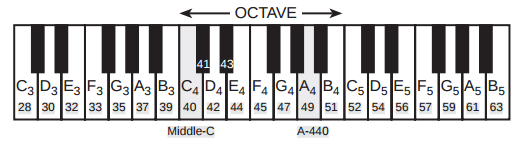
\includegraphics[scale=0.5]{piano.png}
	\caption{Piano keyboard with integer key numbers and reference key $A_4$. Note that not all of the keys are pictured here}
\end{figure}

\begin{figure}[H]
	\centering
	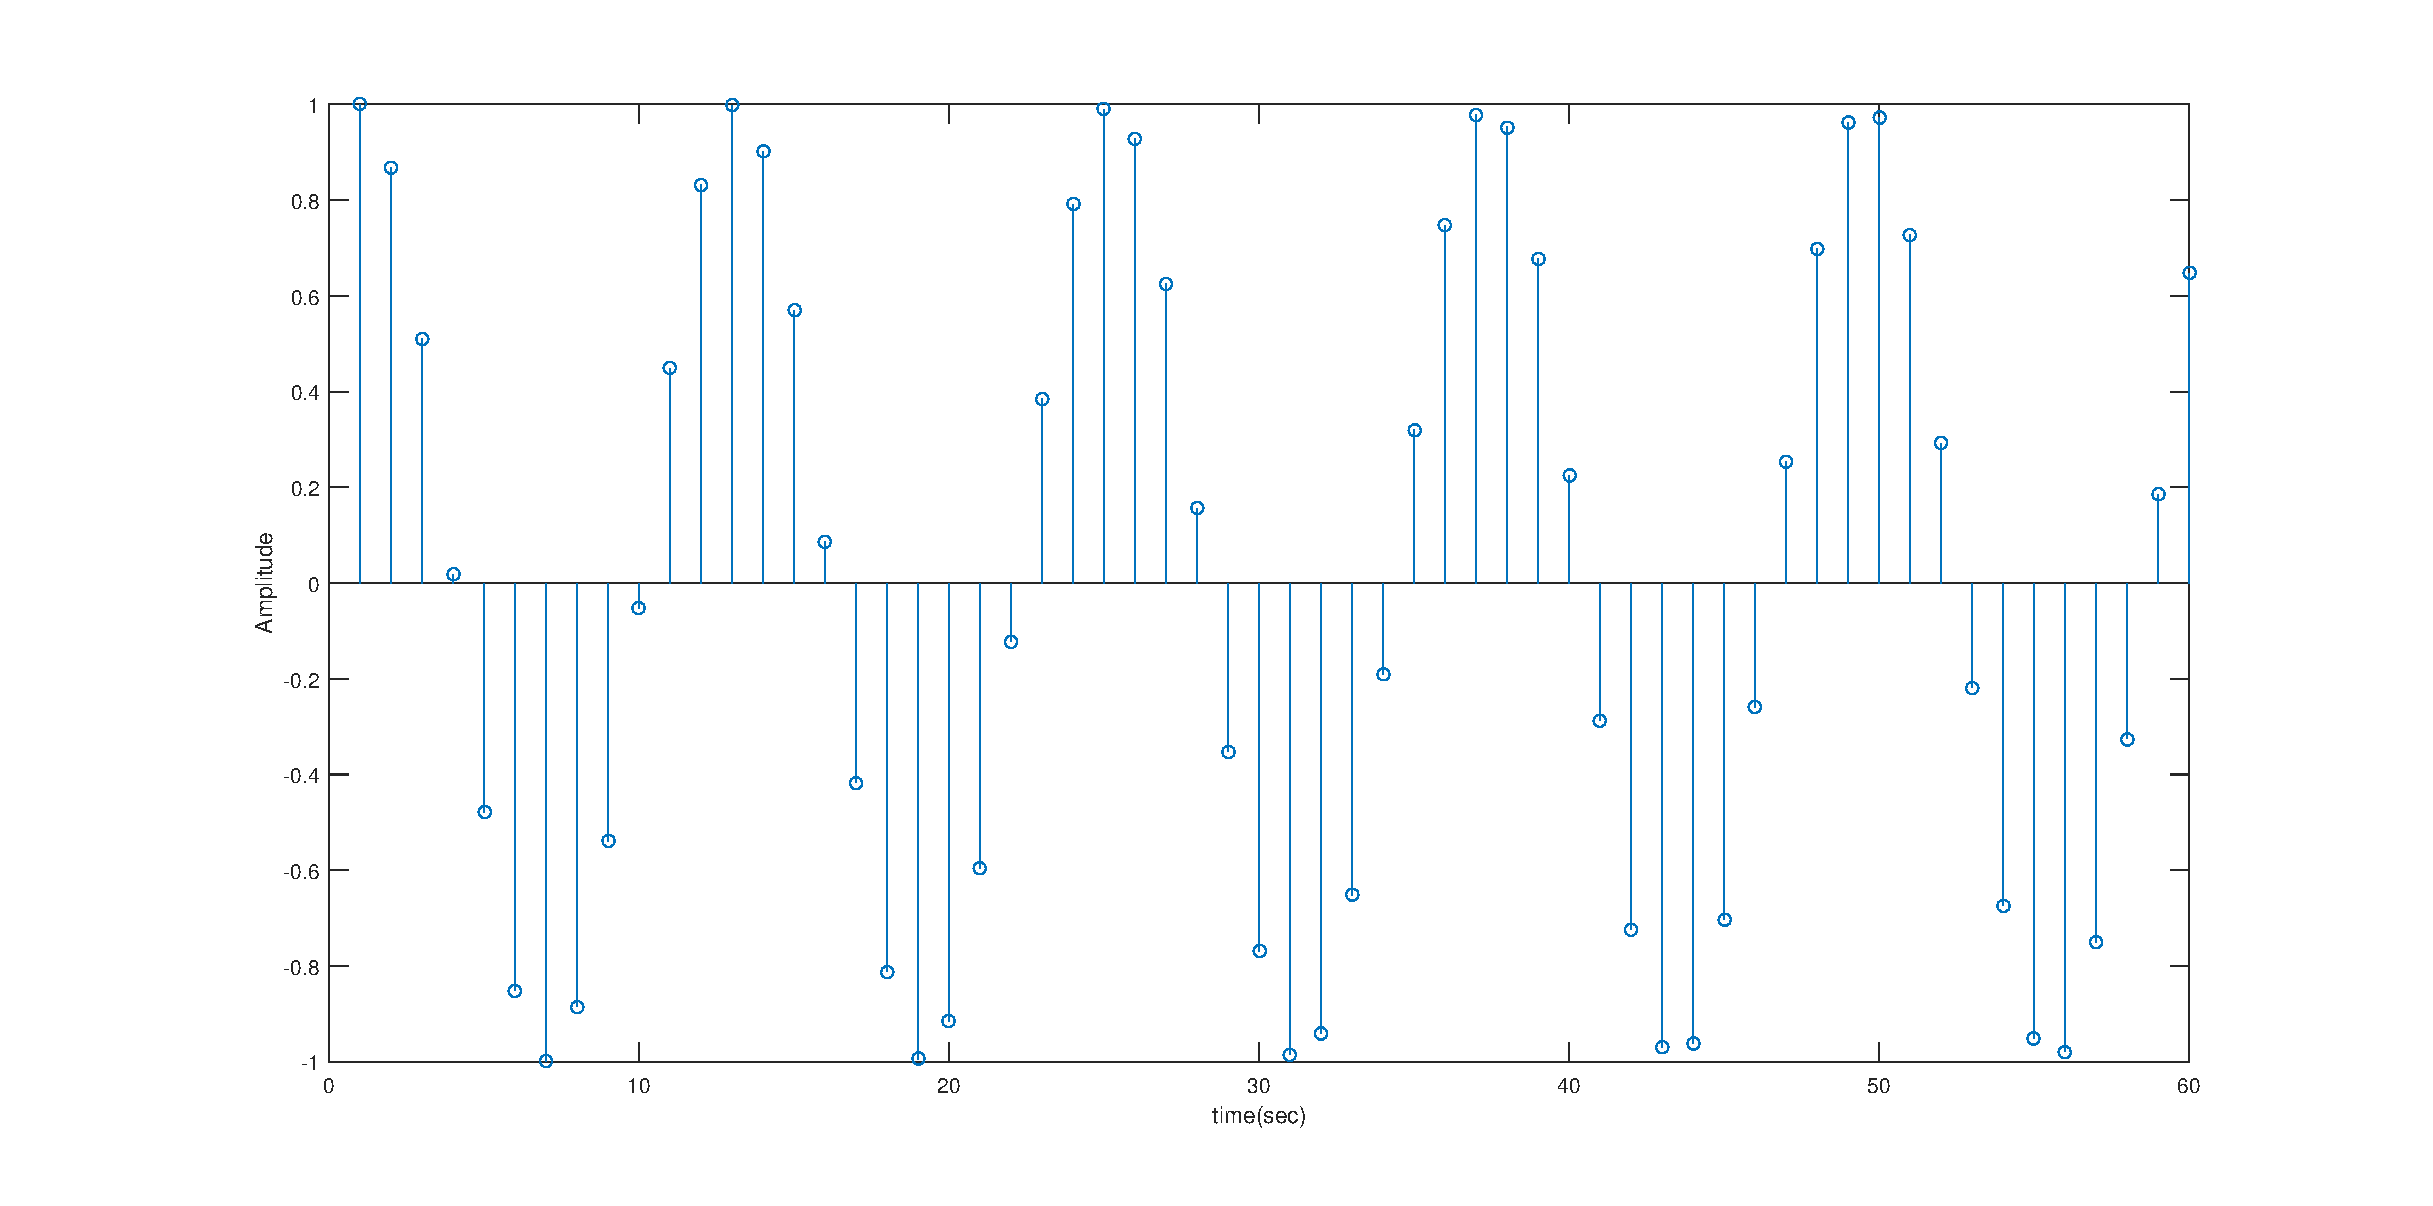
\includegraphics[scale=0.25]{fig2.eps}
	\caption{A temporal plot of the synthesised $A_4$ key}
\end{figure}

In order to play notes on the keyboard a MATLAB function was built, which can be seen in Appendix C. The function takes an argument, \verb|keynum|, which specifies the number of the key that we want to play on the keyboard. The function takes a second argument, \verb|dur|, which specifies the how long the note will be played. A MATLAB script, seen in Appendix D, was written to test the function. The script played a simple scale. It must be noted that the sampling frequency used in this section of the lab was 11025$\si{\hertz}$, recommended by the laboratory instructions.

\newpage

\subsection{Synthesis of \textit{Fur Elise}}
\textit{Fur Elise} is a piece of music composed by Ludwig Van Beethoven which has been synthesised in this laboratory. The implementation of the synthesis, seen in Appendix E, was written in MATLAB and makes use of the previously written note playing function seen in Appendix C. The note sequence and duration for both treble and bass were imported from the file \verb|fenotes.m|. The sampling frequency used for this synthesis is 11025$\si{\hertz}$.


\subsection{Musical Tweaks}
To improve the quality of the synthesised \textit{Fur Elise} two techniques were employed: modulation using an Attack, Decay, Sustain \& Release (ADSR) envelope; and implementing second and third order harmonics.

\subsubsection{ADSR Envelope}
Modulating the signal by some function $E(t)$ is one way in which the sound quality can be improved. Modulating the signal with $E(t)$ means our continuous time output signal is of the form:
\begin{align}
	x(t) = E(t) \cdot \cos(2 \pi f_0 t + \phi)
\end{align}

The recommended choice for the modulation function $E(t)$ was ADSR, the profile of which can be seen in Figure 5. This was implemented using a MATLAB function \verb|adsr_env| which can be seen in Appendix 

\begin{figure}[H]
	\centering
	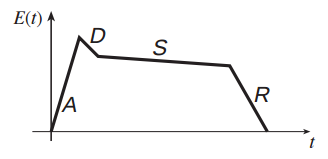
\includegraphics[scale=0.7]{adsr.png}
	\caption{ADSR profile for an envelope function $E(t)$}
\end{figure}

\subsubsection{Second and Third Order Harmonics}
According to McClellan, Schafer \& Yoder (2015), sums of sinusoids used to synthesise periodic signals and that each one of these sinusoids have harmonically related frequencies. That is to say that each sinusoid has some frequency $f_k$ which is multiple of the fundamental frequency $F_0$, for some signal synthesised as:
\begin{align}
	x(t) = A_0 + \sum_{k = 1}^{N}A_k \cos(2 \pi k F_0 t + \phi_k)
\end{align}

Put simply, we have harmonic frequencies which are integer multiples of the :
\begin{align}
	f_k = k F_0
\end{align}

To improve the sound quality of the synthesised notes that individually make up our synthesised \textit{Fur Elise}, it was recommended that the second and third harmonics be introduced. A MATLAB function, making adjustments to the \verb|note| function, implementing the use of harmonics can be seen in Appendix G.
%----------------------------------------------------------------------------------------
%	SECTION 3
%----------------------------------------------------------------------------------------

\section{Improvements}

The theory underlying the task was relatively straight forward and implementation was easy using MATLAB. There were some issues with the amplitude being set to 100 in some of the tasks - this may have been due to some saturation effect on the machine used to conduct the practical. Changing the amplitudes to 1 or lower ensure that lab results fell in line with expectation. 

%----------------------------------------------------------------------------------------
%	BIBLIOGRAPHY
%----------------------------------------------------------------------------------------

\section{References}

McClellan, J.,Schafer, R., \& Yoder, M. (2015). \textit{DSP First} (Global Edition). Harlow, England: Pearson Education Limited.

\newpage
%----------------------------------------------------------------------------------------
%	APPENDIX
%----------------------------------------------------------------------------------------

\section{Appendices}

\subsection{Appendix A}

\begin{lstlisting}
	%%%%%%%%%%%%%%%%%%%%% 2.2 Theory of Sampling %%%%%%%%%%%%%%%%%%%%%%%%
	
	% Clear stored variables and the workspace
	clear; clc;
	
	% Specify the parameters for the task
	A = 100;
	w0_1 = 2*pi*1100;
	ph_1 = 0;
	
	% Specify the sampling rate and the sampling period
	fs = 8000;
	Ts = 1/fs;
	
	% Specify the time vector for the signal duration
	tt = (0:Ts:2);
	
	% The discrete time sample of the analog signal A*cos(w_0*t + ph)
	x1 = A*cos(w0_1*tt + ph_1);
	
	% Listen to the sound of the dsicrete time sampled x1
	sound(x1,fs)
	pause(3);
	
	% The discrete time sample of the analog signal with a phase shift of
	% pi/3 and a different angular frequency
	w0_2 = 2*pi*1650;
	ph_2 = pi/3;
	
	x2 = A*cos(w0_2*tt + ph_2);
	
	% Combining x1 and x2 to listen to them side by side
	xx = [x1 zeros(1,2000) x2];
	sound(xx,fs)
	pause(5)
	
	% Sending the vector xx through the D-A at double the sampling rate
	sound(xx,2*fs)
\end{lstlisting}

\newpage

\subsection{Appendix B}

\begin{lstlisting}
	%%%%%%%%%%%%%%%%%%%%%% 2.3 Piano Keyboard a %%%%%%%%%%%%%%%%%%%%%%%%%%
	% Clear any stored variables and clear the workspace
	clear; clc;
	
	% Initialise the parameters to be used for the script
	A = 100;
	f440 = 440;
	
	% Specify the sampling frequency and sampling period
	fs = 8000;
	Ts = 1/fs;
	
	% Generate the time vector for the discrete points at which the
	% discrete sample will be generated.
	tt = (0:Ts:2);
	
	% Generate the discrete sample of the note
	n = 7;
	fe5 = f440*2^(7/12);
	xx = A*cos(2*pi*fe5*tt);
	
	% Send the note to the D-A converter
	sound(xx,fs)
\end{lstlisting}

\newpage

\subsection{Appendix C}

\begin{lstlisting}
	function tone = note_adv(keynum,dur)
	% NOTE Produce a sinusoidal waveform corresponding to a given
	% piano key number
	
	% usage: tone = note(keynum, dur)
	
	% tone = the output sinusoidal waveform 
	% keynum = the piano keyboard number of the desired note
	% dur = the duration (in seconds) of the output note
	    
	    % Amplitude of the fundamental frequency
	    A0 = 0.5;
	    
	    fs = 11025;
	    tt = 0:(1/fs):dur;
	    
	    if (keynum == 0)
	        tone = 0*tt;
	    else
	        freq0 = 440*2^((keynum-49)/12);
	        freq1 = 2*freq0;
	        freq2 = 3*freq0;
	        
	        tone = A0*cos(2*pi*freq0*tt) ...
	               + 0.75*A0*cos(2*pi*freq1*tt) ...
	               + 0.5*A0*cos(2*pi*freq2*tt);
	    end
	    
	end
\end{lstlisting}

\newpage

\subsection{Appendix D}

\begin{lstlisting}
	%%%%%%%%%%%%%%%%%%%%% 2.3 Piano Keyboard %%%%%%%%%%%%%%%%%%%%%%%%%%%%%%%
	%--- play_scale.m
	clear; clc;
	%---
	keys =    [40 42 44 45 47 49 51 52];
	%--- NOTES: C  D  E  F  G  A  B  C
	% key #40 is middle-C
	%
	dur = 0.25*ones(1,length(keys));
	fs = 11025;
	xx = zeros(1,sum(dur)*fs+1);
	
	n1 = 1;
	
	for kk = 1:length(keys)
	    keynum = keys(kk);
	    
	    tone = note(keynum,0.25);
	    
	    n2 = n1 + length(tone) - 1;
	    xx(n1:n2) = xx(n1:n2) + tone;
	    n1 = n2;
	end
	
	sound(xx,fs)
\end{lstlisting}

\newpage

\subsection{Appendix E}

\begin{lstlisting}
	%%%%%%%%%%%%%%%%%%%%%%%%%%% 3.2 Fur Elise %%%%%%%%%%%%%%%%%%%%%%%%%%%%%
	
	% Clear the workspace and any stored variables
	clear; clc;
	
	% Load the notes and durations for Treble and Bass for Fur Elise
	% from a pre-existing description.
	FENOTES;
	
	% Halve the duration of the notes, because I got sick of listening
	% to this in its original timing
	tdur = tdur/2;
	bdur = bdur/2;
	
	% Specify the sampling frequency used for the D-to-A system
	fs = 11025;
	Ts = 1/fs;
	
	% Synthesize the treble waveform as a combination of sinusoids
	xxt = zeros(1,sum(tdur)*fs+1);
	
	n1 = 1;
	
	for kk = 1:length(t)
	    
	    tone_t = note_adv(t(kk),tdur(kk));
	    E = adsr_env(tone_t);
	    tone_t = E.*tone_t;
	    
	    n2 = n1 + length(tone_t) - 1;
	    xxt(n1:n2) = xxt(n1:n2) + tone_t;
	    n1 = n2;
	end
	
	% Synthesize the bass waveform as a combination of sinusoids
	xxb = zeros(1,sum(bdur)*fs+1);
	
	n1 = 1;
	
	for kk = 1:length(b)
	    
	    tone_b = note_adv(b(kk),bdur(kk));
	    E = adsr_env(tone_b);
	    tone_b = E.*tone_b;
	    
	    n2 = n1 + length(tone_b) - 1;
	    xxb(n1:n2) = xxb(n1:n2) + tone_b;
	    n1 = n2;
	end
	
	% Create the overall waveform
	xx = xxt + xxb;
	
	sound(xx,fs)
\end{lstlisting}

\newpage

\subsection{Appendix F}

\begin{lstlisting}
	function E = adsr_env(tone)
	% Function produces an Attack, Decay, Sustain, Release envelope
	% which we modulate with our signal to provide better sounding tones
	
	    A = linspace(0, 0.6, (length(tone)*0.2)); %rise 20% of signal
	    D = linspace(0.6, 0.5,(length(tone)*0.05)); %drop of 5% of signal
	    S = linspace(0.5, 0.5,(length(tone)*0.4)); %delay of 40% of signal
	    R = linspace(0.5, 0,(length(tone)*0.35)); %drop of 35% of signal
	    
	    ADSR = [A D S R] ; %make a matrix
	
	    len = length(tone) - length(ADSR); %find out the difference
	    
	    %concatenates a horrizontal (2) ADSR + the difference of ADSR
	    % and the signal
	    E = cat(2, ADSR, zeros(1,len));
	end
\end{lstlisting}

\newpage

\subsection{Appendix G}

\begin{lstlisting}
	function tone = note_adv(keynum,dur)
	% NOTE Produce a sinusoidal waveform corresponding to a given
	% piano key number
	
	% usage: tone = note(keynum, dur)
	
	% tone = the output sinusoidal waveform 
	% keynum = the piano keyboard number of the desired note
	% dur = the duration (in seconds) of the output note
	    
	    % Amplitude of the fundamental frequency
	    A0 = 0.5;
	    
	    fs = 11025;
	    tt = 0:(1/fs):dur;
	    
	    if (keynum == 0)
	        tone = 0*tt;
	    else
	        freq0 = 440*2^((keynum-49)/12);
	        freq1 = 2*freq0;
	        freq2 = 3*freq0;
	        
	        tone = A0*cos(2*pi*freq0*tt) ...
	               + 0.75*A0*cos(2*pi*freq1*tt) ...
	               + 0.5*A0*cos(2*pi*freq2*tt);
	    end
	    
	end
\end{lstlisting}
%----------------------------------------------------------------------------------------


\end{document}